% !TEX root = ../../lectures.tex
\section{Alfv\'en waves through a mechanical analogy}

Consider a uniform, perfectly conducting plasma at rest with a uniform magnetic field
\(\mathbf B_0\).
In ideal MHD the field is \emph{frozen} into the fluid, so a small sideways nudge of a fluid element relative to \(\mathbf B_0\) bends the field lines. Bending stores magnetic energy, and the field responds with a \emph{tension} that tries to straighten the lines. This tension provides the restoring force that launches a disturbance along \(\mathbf B_0\).

It is convenient to write the magnetic force per unit volume (the magnetic force density) as
\[
\mathbf f
= \frac{1}{4\pi}(\mathbf B\!\cdot\!\nabla)\mathbf B
\;-\;\nabla\!\left(\frac{B^2}{8\pi}\right).
\]

The second term acts like an isotropic \emph{magnetic pressure}; the first is the \emph{magnetic tension} that pulls along the field direction. If a field line is bent with radius of curvature \(R\), the tension generates a transverse restoring force of order
\[
f_\perp \sim \frac{B_0^2}{4\pi}\,\frac{1}{R},
\]
precisely the behavior of a taut string that resists curvature!

To make this analogy quantitative, take a thin magnetic \emph{flux tube} of cross-section \(A\) following \(\mathbf B_0\), and let \(s\) be arc length along the unperturbed field. A small transverse displacement \(\xi_\perp(s,t)\) introduces curvature \(\kappa \approx \partial_s^2 \xi_\perp\).
The tension acting on a short segment of length \(\Delta s\) is then
\[
F_\perp \;=\; \Big(\frac{B_0^2}{4\pi}\Big) A\,\frac{\partial^2 \xi_\perp}{\partial s^2}\,\Delta s,
\]
because the field exerts a tension \(B_0^2/4\pi\) per unit area along the tube.
The segment’s mass is \(\rho\,A\,\Delta s\), so Newton’s second law gives
\[
\rho A\,\Delta s\,\frac{\partial^2\xi_\perp}{\partial t^2}
\;=\;
\Big(\frac{B_0^2}{4\pi}\Big) A\,\frac{\partial^2 \xi_\perp}{\partial s^2}\,\Delta s.
\]
Canceling \(A\Delta s\) yields the transverse wave equation
\[
\frac{\partial^2\xi_\perp}{\partial t^2}
\;=\;
\frac{B_0^2}{4\pi\rho}\,\frac{\partial^2\xi_\perp}{\partial s^2}.
\]

At this point the identification with the vibrating string is immediate. The string equation
\(\partial_t^2 \xi = (T/\mu)\,\partial_s^2 \xi\)
involves a \emph{tension} \(T\) and a \emph{linear mass density} \(\mu\).
For our flux tube,
\[
T=\frac{B_0^2}{4\pi}\,A,
\quad \text{and} \quad
\mu=\rho\,A,
\]
so that \(T/\mu = B_0^2/(4\pi\rho)\).
The solution of the string equation is given in terms of a wave with speed
\begin{remark}
\[
v_A \;=\; \sqrt{\tfrac{T}{\mu}} \;=\; \frac{B_0}{\sqrt{4\pi\rho}}
\]
\end{remark}
%Notice how the cross-section \(A\) cancels: only \(B_0\) and \(\rho\) matter.

\begin{figure}[t] 
\centering 
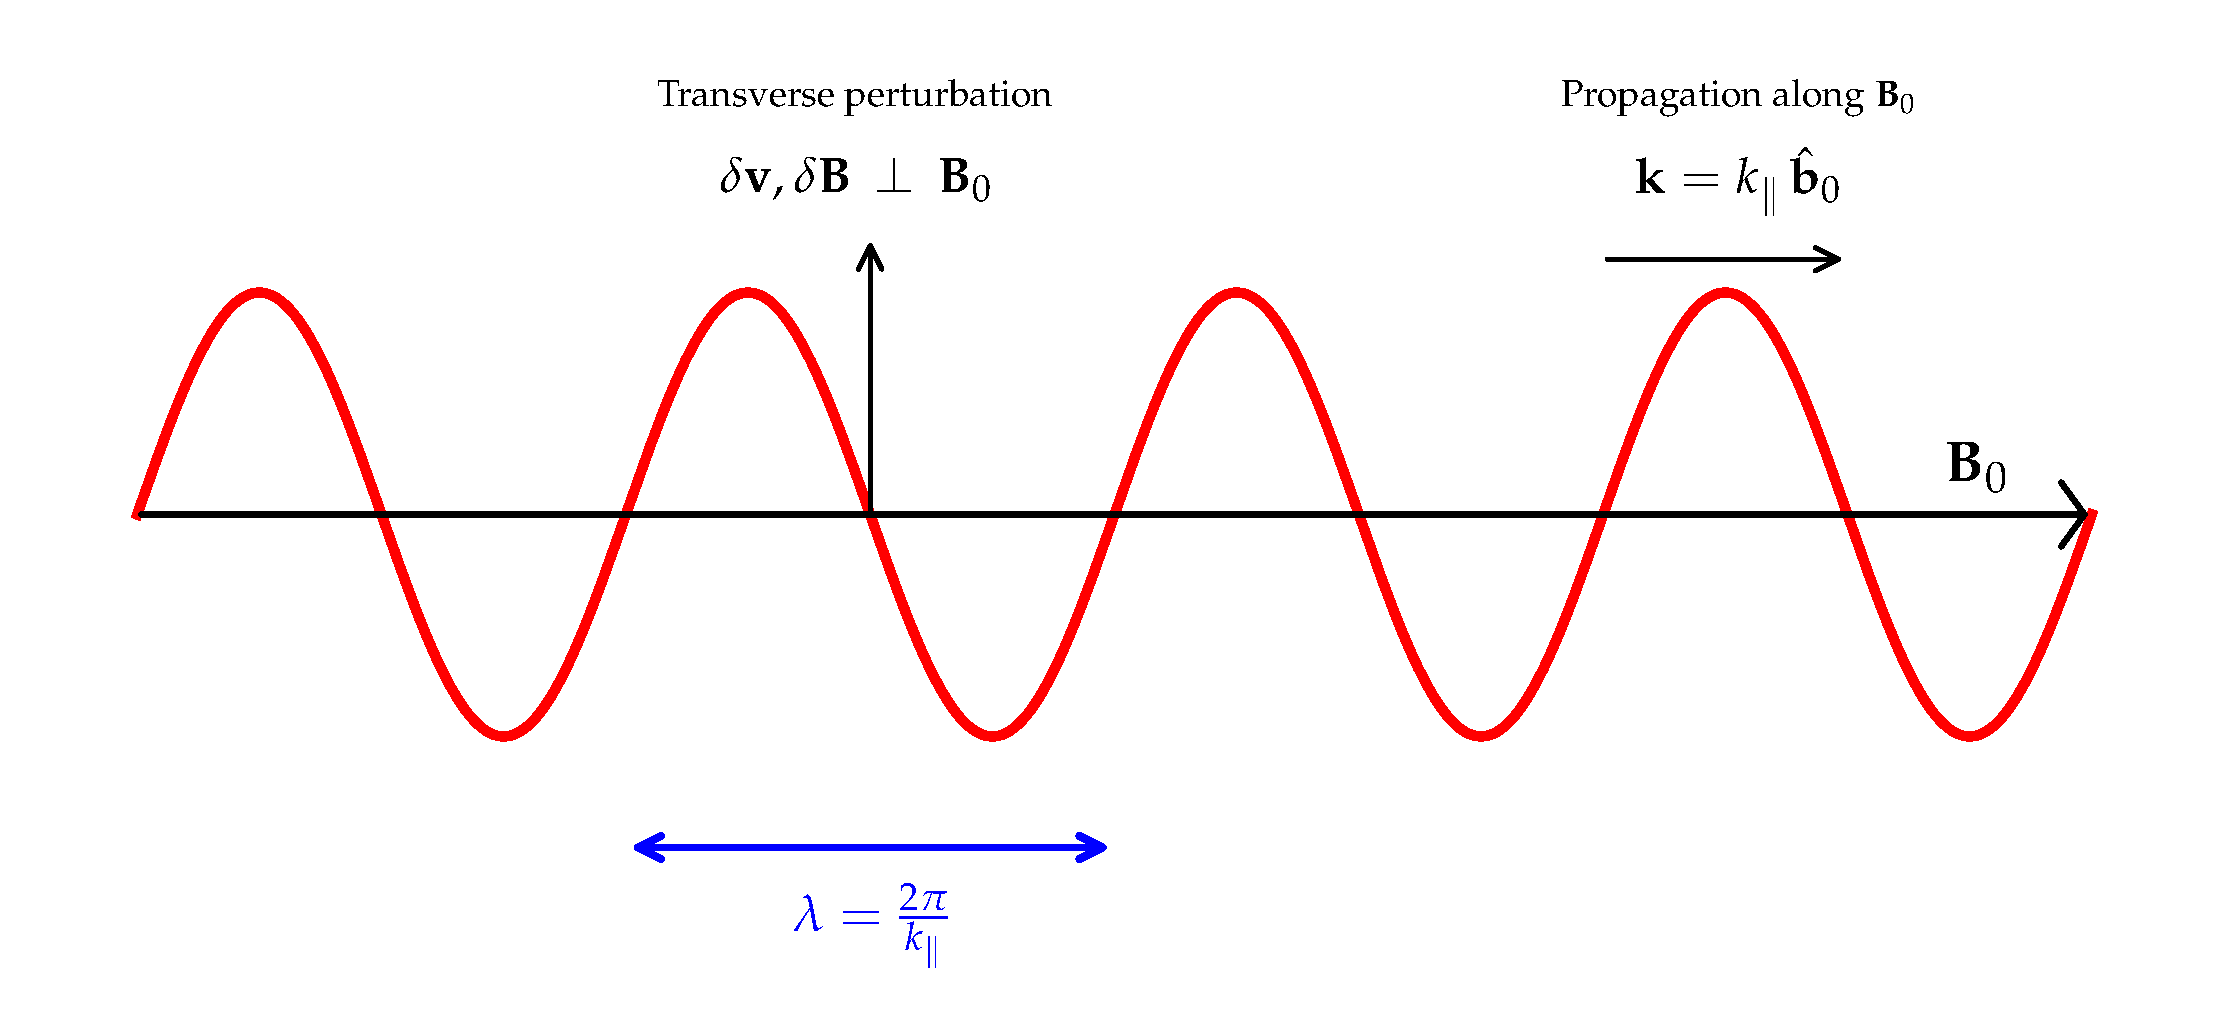
\includegraphics[width=\textwidth]{figures/alfven_diagram.pdf}
\caption{.} 
\label{fig:alfvenwave} 
\end{figure}

Why does an Alfvén disturbance propagate \emph{along} \(\mathbf B_0\)?
Because the restoring force is magnetic \emph{tension}—it arises from field-line curvature, which requires variation \emph{along} the field. If the wavevector has no component along \(\mathbf B_0\) (\(k_\parallel=0\)), the field lines are not bent and the tension vanishes to leading order: there is no shear-Alfvén propagation. In the linear regime this is reflected by the dispersion relation
\[
\omega=\pm k_\parallel v_A,
\]
which depends only on the parallel component of the wavevector.

Energetically, the picture mirrors the lossless string: as the wave oscillates, magnetic bending energy converts into kinetic energy and back again, with equal time-averaged contributions. The magnetic-pressure term is unchanged to leading order for a pure Alfvén mode; it is the tension piece that does the “work”.

\begin{remark}{Characteristic speeds in ISM}

For the Alfv\'en speed in the ISM we use
\[
v_A \simeq \frac{B}{\sqrt{4\pi\,\rho}}
\;\approx\;
\frac{B}{\sqrt{4\pi\,m_p\,n_i}},
\]
where \(n_i\) is the ion number density.  
In the warm ISM, taking \(B \sim 5~\mu\mathrm{G}\) and \(n_i \sim 1~\mathrm{cm^{-3}}\) gives
\[
v_A \sim 10\text{--}20~\mathrm{km\,s^{-1}}.
\]
This is tiny compared with relativistic particle speeds, so cosmic rays (with \(v\simeq c\)) effectively \emph{see} Alfv\'en waves as stationary scattering centers in many Galactic environments.

For comparison, the adiabatic sound speed
%\[
%c_s=\sqrt{\frac{\gamma k_B T}{\mu m_p}}
%\]
is \(c_s \approx 10~\mathrm{km\,s^{-1}}\) for a typical warm ISM temperature \(T\!\sim\!8000~\mathrm{K}\) (with reasonable \(\mu\) and \(\gamma\)). Thus Alfv\'en and sound speeds are of the same order, implying a plasma beta
\[
\beta \equiv \frac{8\pi p}{B^2} \sim \mathcal O (1)
\]
near unity in these phases.

In the \emph{solar corona}, the parameters are very different: \(B_0\!\sim\!10~\mathrm{G}\) and \(n\!\sim\!10^9~\mathrm{cm^{-3}}\) yield
\( 
v_A \approx 690~\mathrm{km\,s^{-1}},
\)
typically much larger than \(c_s\) there, i.e.\ \(\beta \ll 1\). In short: the warm ISM is a \(\beta\!\sim\!1\) environment with \(v_A\!\sim\!c_s\), whereas the corona is tension-dominated with \(v_A\!\gg\!c_s\).
\end{remark}

%\subsection{Alfv\'en Waves (vs.\ Sound Waves)}
%
%\paragraph{Setting and assumptions.}
%We work in (ideal) MHD with a uniform equilibrium:
%\[
%\mathbf{B}_0=\text{const},\qquad \rho_0=\text{const},\qquad \mathbf{v}_0=\mathbf{0},\qquad p_0=\text{const}.
%\]
%Small perturbations $\delta \rho,\,\delta p,\,\delta \mathbf{v},\,\delta \mathbf{B}$ vary as $\exp[i(\mathbf{k}\!\cdot\!\mathbf{x}-\omega t)]$.
%The ideal MHD equations we linearize are
%\[
%\begin{aligned}
%&\partial_t \rho + \nabla\!\cdot(\rho \mathbf{v}) = 0,\\
%&\rho\,\partial_t \mathbf{v} = -\nabla p + \frac{1}{\mu_0}(\nabla\times \mathbf{B})\times \mathbf{B},\\
%&\partial_t \mathbf{B} = \nabla\times(\mathbf{v}\times \mathbf{B}),\qquad \nabla\!\cdot\!\mathbf{B}=0,\\
%&\delta p = c_s^2\,\delta \rho\quad(\text{adiabatic closure, }c_s^2=\gamma p_0/\rho_0).
%\end{aligned}
%\]
%
%\paragraph{Alfv\'en waves: definition and dispersion.}
%Alfv\'en waves are \emph{transverse, incompressible} MHD waves whose restoring force is the magnetic tension of the background field $\mathbf{B}_0$.
%They satisfy
%\[
%\delta \rho = 0,\qquad \delta p = 0,\qquad \mathbf{k}\cdot \delta\mathbf{v}=0,
%\]
%with polarization $\delta\mathbf{v}\perp\mathbf{B}_0$ and $\delta\mathbf{B}\perp\mathbf{B}_0$.
%Writing $\mathbf{k}=k_\parallel \hat{\mathbf{b}}_0 + \mathbf{k}_\perp$ with $\hat{\mathbf{b}}_0=\mathbf{B}_0/B_0$, the dispersion relation is
%\[
%\boxed{\ \omega = \pm k_\parallel v_A\ ,\qquad v_A=\frac{B_0}{\sqrt{\mu_0 \rho_0}}\ } \quad
%\text{(SI)}\qquad\text{or}\qquad v_A=\frac{B_0}{\sqrt{4\pi \rho_0}}\ \text{(cgs)}.
%\]
%Key features:
%\begin{itemize}
%\item Propagate \emph{along field lines}: no propagation if $k_\parallel=0$.
%\item \emph{Transverse} polarization: $\delta\mathbf{v}\perp \mathbf{k}$ and $\delta\mathbf{v}\perp \mathbf{B}_0$ (shear Alfv\'en mode).
%\item \emph{Incompressible}: no density/pressure perturbations at leading order.
%\item Energy equipartition in linear waves: kinetic and magnetic perturbation energies are equal on average.
%\item Group and phase velocities are $\pm v_A\,\hat{\mathbf{b}}_0$ (purely along $\mathbf{B}_0$).
%\end{itemize}
%
%\paragraph{Physical picture.}
%Imagine a taut magnetic ``string'' (field line). A sideways displacement bends it, creating curvature and a \emph{tension} force $\propto B_0^2$ that pulls the plasma back; inertia is provided by $\rho_0$. The wave speed therefore scales as $v_A\propto B_0/\sqrt{\rho_0}$.
%
%\paragraph{Sound waves: contrast.}
%Ordinary sound waves in a neutral or weakly magnetized fluid have
%\[
%\boxed{\ \omega = \pm k\,c_s\ ,\qquad \delta\mathbf{v}\parallel \mathbf{k}\ ,\qquad \text{compressive}~(\delta\rho,\delta p\neq 0)\ }.
%\]
%They are longitudinal, isotropic (no preferred direction), and the restoring force is the \emph{gas pressure gradient}, not magnetic tension.
%
%\paragraph{Magnetized plasma taxonomy (for context).}
%In a magnetized plasma there are three linear MHD modes:
%\begin{enumerate}
%\item \textbf{Alfv\'en} (transverse, incompressible, $\omega=\pm k_\parallel v_A$).
%\item \textbf{Slow magnetosonic} (compressive, generally sub-$\min\{c_s,v_A\}$, strongly field-aligned at low $\beta$).
%\item \textbf{Fast magnetosonic} (compressive, more isotropic, super-$\max\{c_s,v_A\}$ at low $\beta$).
%\end{enumerate}
%The relative importance of these modes depends on the plasma beta
%\[
%\beta \equiv \frac{2\mu_0 p_0}{B_0^2} \quad \text{(SI)}\qquad \Big(\text{or } \beta=8\pi p_0/B_0^2\ \text{in cgs}\Big).
%\]
%Low-$\beta$ plasmas ($\beta\ll1$) are tension-dominated ($v_A\gg c_s$); high-$\beta$ plasmas behave more like ordinary fluids ($c_s\gtrsim v_A$).
%
%\paragraph{Polarization and correlations.}
%For linear Alfv\'en waves,
%\[
%\delta\mathbf{B} = \pm \sqrt{\mu_0 \rho_0}\,\delta\mathbf{v}\times \hat{\mathbf{b}}_0,\qquad
%\delta\mathbf{E} = -\,\delta\mathbf{v}\times \mathbf{B}_0,
%\]
%and the Poynting flux $\mathbf{S}=\mu_0^{-1}\,\delta\mathbf{E}\times \delta\mathbf{B}$ points along $\pm\hat{\mathbf{b}}_0$.
%
%\paragraph{Damping (very brief).}
%Ideal MHD is dissipationless. In real plasmas, Alfv\'en waves can damp via:
%viscosity/resistivity (Ohmic), ion–neutral friction (partially ionized media), phase mixing and resonant absorption (inhomogeneous $v_A$), and at smaller scales via kinetic effects (e.g.\ Landau/cyclotron damping; ``kinetic Alfv\'en'' regime when $k_\perp \rho_i\!\sim\!1$).
%%
%\paragraph{Worked numbers.}
%\begin{itemize}
%\item \emph{Warm ISM:} $B_0\!\sim\!5~\mu\text{G}$, $n\!\sim\!1~\text{cm}^{-3}$ $\Rightarrow$ 
%$v_A \approx 2.18\,\frac{B_{[\mu\text{G}]}}{\sqrt{n_{[\text{cm}^{-3}]}}}\,\text{km s}^{-1} \approx 11~\text{km s}^{-1}$.
%For $T\!\sim\!8000$ K, $c_s\!\approx\!9~\text{km s}^{-1}$, so Alfv\'en and sound speeds are comparable.
%\item \emph{Solar corona:} $B_0\!\sim\!10~\text{G}$, $n\!\sim\!10^9~\text{cm}^{-3}$ $\Rightarrow$
%$v_A \approx 2.18\,\frac{10^7}{\sqrt{10^9}} \approx 690~\text{km s}^{-1}$, typically $\gg c_s$ ($\beta\ll1$).
%\end{itemize}
%
%\paragraph{At-a-glance comparison.}
%\begin{center}
%\begin{tabular}{lcc}
%\toprule
% & \textbf{Alfv\'en wave} & \textbf{Sound wave} \\
%\midrule
%Restoring force & Magnetic tension ($\propto B_0^2$) & Gas pressure gradient \\
%Compressibility & Incompressible ($\delta \rho=0$) & Compressive ($\delta \rho\neq 0$) \\
%Polarization & Transverse ($\delta\mathbf{v}\perp \mathbf{k},\mathbf{B}_0$) & Longitudinal ($\delta\mathbf{v}\parallel \mathbf{k}$) \\
%Dispersion & $\omega=\pm k_\parallel v_A$ & $\omega=\pm k\,c_s$ \\
%Anisotropy & Propagates along $\mathbf{B}_0$ & Isotropic \\
%Energy flux & Along field lines & Along $\mathbf{k}$ \\
%Key parameter & $v_A=B_0/\sqrt{\mu_0\rho_0}$ & $c_s=\sqrt{\gamma p_0/\rho_0}$ \\
%\bottomrule
%\end{tabular}
%\end{center}
%
%\paragraph{Derivation sketch.}
%Taking $\mathbf{k}$ in the $x$–$z$ plane with $\mathbf{B}_0=B_0\hat{\mathbf{z}}$ and seeking a transverse solution with $\delta v_y\neq 0$, the linearized momentum and induction equations give
%\[
%-i\omega \rho_0\,\delta v_y = \frac{i k_\parallel B_0}{\mu_0}\,\delta B_y,\qquad
%-i\omega\,\delta B_y = i k_\parallel B_0\,\delta v_y,
%\]
%which combine to yield $\omega^2 = k_\parallel^2 v_A^2$ and the phase relation 
%$\delta B_y = \pm \sqrt{\mu_0\rho_0}\,\delta v_y$.
%
%\paragraph{Where they matter.}
%Alfv\'en waves are ubiquitous in magnetized astrophysical plasmas: solar wind/corona, planetary magnetospheres, interstellar turbulence, and accretion/ejection environments. They mediate energy and momentum transport along field lines and are central to plasma heating, turbulence cascades, and cosmic-ray scattering.
%
%\paragraph{Exercises.}
%\begin{enumerate}
%\item Show that the time-averaged kinetic and magnetic perturbation energies of a linear Alfv\'en wave are equal.
%\item For a plasma with $\beta=0.1$ and $c_s=100~\text{km s}^{-1}$, estimate $v_A$ and discuss which linear mode transports energy most efficiently across vs.\ along the mean field.
%\item Starting from the linearized MHD system, derive the full magnetosonic dispersion relation for arbitrary angle between $\mathbf{k}$ and $\mathbf{B}_0$, and identify the slow/fast branches in the limits $\beta\ll1$ and $\beta\gg1$.
%\end{enumerate}
